 

\documentclass{article}
%%%%%%%%%%%%%%%%%%%%%%%%%%%%%%%%%%%%%%%%%%%%%%%%%%%%%%%%%%%%%%%%%%%%%%%%%%%%%%%%%%%%%%%%%%%%%%%%%%%%%%%%%%%%%%%%%%%%%%%%%%%%



\usepackage{epigraph}
\usepackage[toc,page]{appendix}

\usepackage{graphicx}
\usepackage{subfig}


\usepackage{multirow}

\newcommand{\ns}{\noindent }

\newcommand{\sh}[1]{\indent\indent\texttt{\footnotesize\$ #1}}
\newcommand{\shni}[1]{\texttt{\footnotesize\$ #1}}


 \textwidth = 400pt
 \textheight = 570pt
 \oddsidemargin =0 pt

\usepackage[colorlinks=true]{hyperref}



\begin{document}

    {\bfseries\Large
        Puebla vs Global temperature trends\\
        \vskip1cm
        R. Angeles\\
    }    




\section{SQL Data extraction}

Check the nearest town using

\sh{SELECT city FROM city-list WHERE country = 'Mexico'}

It is Puebla city. Then the local avg temp timeline can be downloaded from

\sh{SELECT year, avg-temp FROM city-data WHERE city = 'Puebla' }

Finally extract global data 

\sh{SELECT * FROM global-data }

\section{Pandas code}

\begin{figure}[!h]
\centering
  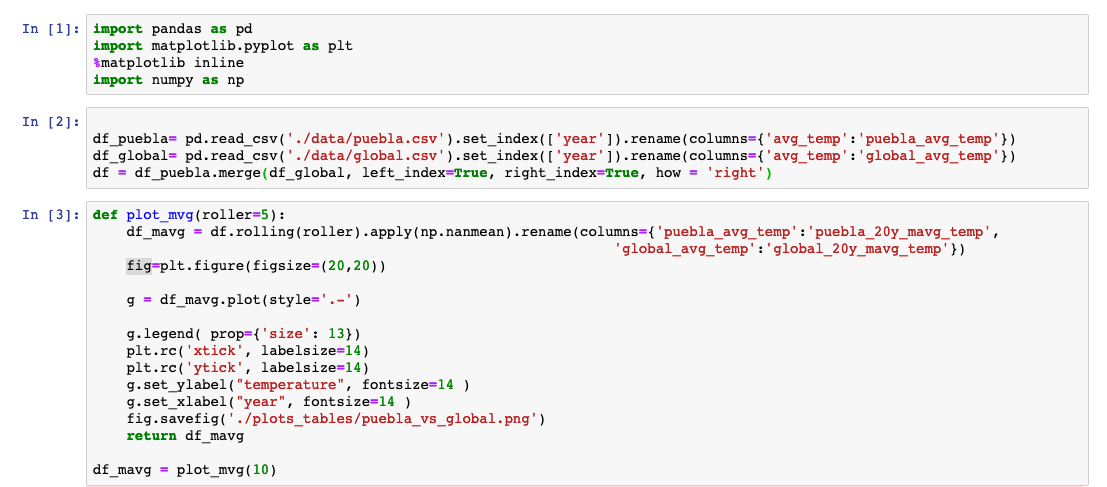
\includegraphics[width=120mm]{../plots_tables/jupyter.png}
%  \caption{Training dataset}
% \label{fig:train_head}
\end{figure}

\section{Running avg temperature}
\begin{figure}[!h]
\centering
  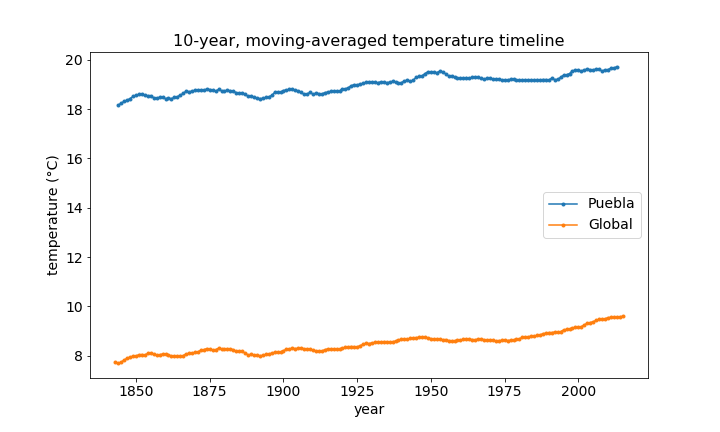
\includegraphics[width=100mm]{../plots_tables/puebla_vs_global.png}
  \caption{Time series, starting at 1834, of the 10 years running averaged temperature.}\label{fig:vs}
\end{figure}


Observations on  Fig.~\ref{fig:vs}:
\begin{itemize}
\item Locally (in Puebla city) and globally the temperature seems to be increasing approximately linearly, plus
fluctuations. The total temperature change seems to be between 1 and 2 degrees. 
\item Fluctuations occur over time scales of a 2 to 5 decades. 
\item The fluctuations in the local and global case are not independent in the sense that they  
have similar shape and occur simultaneously. 
\item In the last 50 years the global temperature seems to increase slightly faster than before, perhaps 
another line with a higher slope. This change is also present in the case of puebla 
but starting more recently, around 1995. 
\end{itemize}

\bibliographystyle{unsrt}
\bibliography{qcd22}

\end{document}
